\documentclass[../main.tex]{subfiles}
\graphicspath{{\subfix{../IMAGES/}}}

\begin{document}
\localtableofcontents

\subsection{Représentation binaire}
\warning Lors du travail en binaire, on effectue des additions modulaire, risque de dépassement de capacité.\\

On peut alors représenter les valeurs possible sur une roue.\\

\begin{figure}[hbt!]
    \centering
    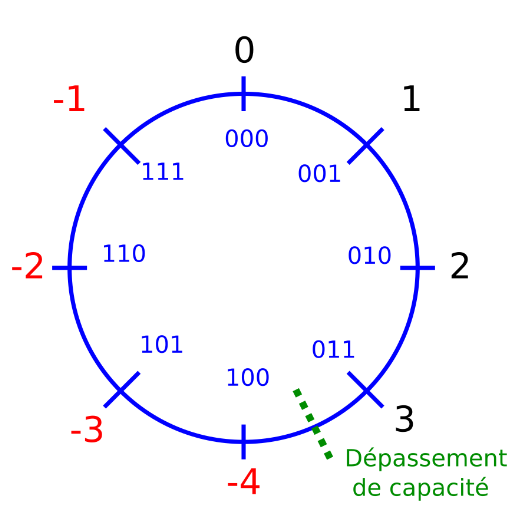
\includegraphics[width=.5\textwidth]{IMAGES/elec/Screenshot from 2024-02-29 11-40-53.png}
\end{figure}

On peut également représenter des nombres signés (bit de signe).\\

Types en C : \begin{itemize}
    \item char : nombre de 8 bits\\
    \item signed char : 8bits signés\\
    \item unsigned char : 8bits positifs\\
    \item int : généralement 16 bits (dépend de la machine)\\
    \item signed int : 16 bits signés\\
    \item unsigned int : 16 bits positifs\\
    \item long int : généralement 32 bits\\
    \item signed long int : 32 bits signés\\
    \item unsigned long int : 32 bits positifs\\
\end{itemize}

Il est préférable d'utiliser les dénominations : \begin{itemize}
    \item uint8\_t : 8 bits positifs (0 - 255)\\
    \item int8\_t : 8 bits signés (-128 - 127)\\
    \item uint16\_t : 16 bits positifs (0 65635)\\
    \item int16\_t : 16 bits signés (-32768 - 34767)\\
    \item uint32\_t : 32 bits positif (0 - 4294967295)\\
    \item int32\_t : 32 bits signés (-2147483648 - 2147483647)\\
\end{itemize}

\subsection{Gestion du temps}
\subsubsection{Gérer les sorties}
La durée d'une instruction est courte (de l'ordre de la micro seconde).\\
Pour une boucle de délai, on emploi une variable de type volatile int !\\

\warning Les attentes sont bloquantes.\\
Il faut donc avoir une boucle principale à durée constante et ne pas utiliser de boucles à l'intérieur.\\

\subsubsection{Gérer les entrées}
Le passeur d'entrée ne donne la valeur qu'à l'instant de la lecture. \textbf{La scrutation (polling)} est l'examen répété de l'état d'un ou plusieurs éléments d'un système.\\

La fréquence d'échantillonnage doit être au minimum 2 fois la fréquence maximale d'entrée !\\

\subsection{Entrée/sorties}
\begin{itemize}
    \item Set bit : P1DIR |= (1<<6); (on définit la valeur de P1.6 a 1)\\
    \item Clear bit : P1OUT \&=$\Tilde{}$(1<<6); (on définit la valeur de P1.6 a 0)\\
\end{itemize}

\subsubsection{Résistances de tirage}
Une résistance reliée à une alimentation assure un potentiel connu : Pull-up (vers le haut) et Pull-down (vers le bas).\\

On a dès lors : \begin{table}[hbt!]
    \centering
    \begin{tabular}{|c|c|c|c|}
    \hline
        Ren & Dir & Out & Rôle de la patte \\ \hline
        0 & 0 & 0 & Entrée\\ \hline
        1 & 0 & 1 & Entrée en Pull-up\\ \hline
        1 & 0 & 0 & Entrée en Pull-down\\ \hline
        0 & 1 & 0 & Sortie à 0\\ \hline
        0 & 1 & 1 & Sortie à 1\\ \hline
    \end{tabular}
\end{table}

Le registre PxREN enclenche la résistance, PxDIR donne le sens de la patte.\\

\subsection{PWM}
Pulse Width Modulation.\\
Sur une période, le signal est actif avec une largeur d'impulsions puis il est inactif sur le temps restant.\\

Cela va du Hz à des dizaines de MHz (période minimale pour voir à l'oeil nu : 20ms, 50Hz).\\

\subsection{Interruptions}
On peut remplacer la scrutation par des interruptions (beaucoup plus efficace et sur). Le programme principal s'arrête le temps de l'exécution de l'interruption. \\
Plusieurs possibilités : \begin{itemize}
    \item P1IE : Interrupt Enable\\
    \item P1IES : Interrupt Edge Select (1 : front descendant, 0 : front montant)\\
    \item P1IFG : Interrupt FlaG (1 si interruption détecté)\\
\end{itemize}

Ils sont tous encodés en 8bits. \warning Remettre le fanion d'interruption à 0 après la détection d'une interruption.\\

Ecriture : (interruption sur port 1.3) \\
int main()\{\\
\qquad P1IES |= (1<<3); (front descendant)\\
\qquad P1IE |= (1<<3); (interruption sur P1.3)\\
\qquad P1IFG \&=$\sim$ (1<<3); (fanion à 0)\\
\qquad \_\_enable\_interrupt();\\
\qquad while(1) \{\\
\}\\
\}\\
\#pragma vector=PORT1\_VECTOR (routine d'interruption)\\
\_\_interrupt void Port1\_ISR(void)\{\\
\qquad P1IFG \& = $\sim$(1<<3); (remise à 0 du fanion)\\
\}\\


\subsection{Timers}
On peut obtenir une gestion du temps très précise à l'aide des timers qui utilisent un signal oscillateur afin de compter.\\

\begin{figure}[hbt!]
    \centering
    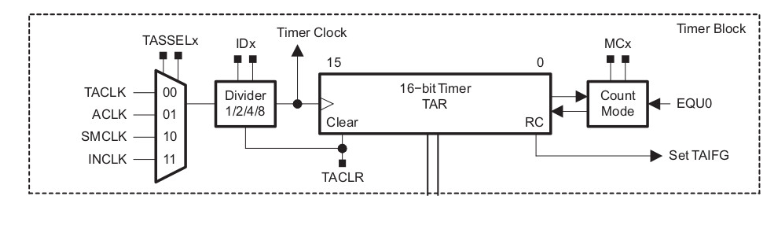
\includegraphics[width=.7\textwidth]{IMAGES/proddev/Screenshot from 2024-04-25 10-49-21.png}
    \caption{Timer A du MSP430}
\end{figure}

\subsubsection{Registre de contrôle}
Il s'agit d'une valeur 16 bits contenant : \begin{itemize}
    \item Bits 15-10 : unused\\
    \item Bits 9-8 : \textbf{TASSELx} Timer\_ A clock source select \begin{itemize}
        \item 00 : TACLK\\
        \item 01 : ACLK\\
        \item 10 : SMCLK(system clock, most precise one)\\
        \item 22 : INCLK\\
    \end{itemize}
    \item Bits 7-6 : \textbf{IDx} input divider \begin{itemize}
        \item 00 : /1\\
        \item 01 : /2\\
        \item 10 : /4\\
        \item 11 : /8\\
    \end{itemize}
    \item Bits 5-4 : \textbf{MCx} mode control \begin{itemize}
        \item 00 : stop mode\\
        \item 01 : up-mode (counts up to TACCR0)\\
        \item 10 : continuous mode (counts to 0FFFFh, maximum and then overflow)\\
        \item 11 : up/down mode (counts up to TACCR0 and down)\\
    \end{itemize}
    \item Bit 3 : unused\\
    \item Bit 2 : \textbf{TACLR} Timer\_A clear\\
    \item Bit 1 : \textbf{TAIE} Timer\_A interrupt enable\\
    \item Bit 0 : \textbf{TAIFG} Timer\_A interrupt flag\\
\end{itemize}


\subsubsection{Registre de comparaison}
On cherche ici à trouver une valeur spécifique dans le timer pour déclancher.\\

\begin{itemize}
    \item Bit 4 : \textbf{CCIE} capture/compare interrupt enable\\
    \item Bit 3 : \textbf{CCI} capture/compare input (used to read the input)\\
    \item Bit 2 : \textbf{OUT} controls the state of the output\\
    \item Bit 1 : \textbf{COV} capture overflow \warning MUST BE RESETTED MANUALLY\\
    \item Bit 0 : \textbf{CCIFG} capture/compare interrupt flag\\
\end{itemize}


\end{document}